\documentclass[10pt,twocolumn]{article}

\usepackage[a4paper,margin=2.1cm,columnsep=0.75cm]{geometry}
\usepackage{amsmath,amssymb,amsthm,mathtools}
\usepackage{booktabs}
\usepackage{float}
\usepackage{tikz}
\usepackage[colorlinks=true,linkcolor=blue!60!black,citecolor=blue!60!black,urlcolor=blue!60!black]{hyperref}

\usetikzlibrary{arrows.meta,positioning}

\floatstyle{ruled}
\newfloat{algorithm}{tbp}{loa}
\floatname{algorithm}{Algorithm}
\renewcommand{\labelitemi}{$\bullet$}

\newtheorem{proposition}{Proposition}
\newtheorem{remark}{Remark}

\newcommand{\dman}{d_{\mathrm{Man}}}
\newcommand{\eps}{\varepsilon}

\title{\bfseries Routing an Ambulance through a Grid-Structured City:\\ Integer Programming, Sensitivity Analysis, $A^{\star}$ Search\\[2mm]
\large A Two-Leg Shortest Path Project on Manhattan-Plan Road Networks}

\author{Lampros Printzios\\
{\small ECE Department, University of Patras, Greece, \texttt{printzios\_lampros@ac.upatras.gr}}\\
{\small Final project for the course ``Linear and Combinatorial Optimization''}}
\date{}

\begin{document}

\maketitle

\begin{abstract}
\noindent
We study a two-leg ambulance routing problem on city road networks with a rectangular
(Manhattan) street plan: an ambulance must first reach a patient and then transport the patient
to a hospital, so that each leg is a single-pair shortest path problem on a directed,
edge-weighted grid network. Each leg is modeled as a minimum-cost-flow-type integer program
(IP) with binary arc variables and flow-conservation constraints, which is solved with the
GLPK solver through the \textsf{pymprog} modeling layer. We establish several structural
properties of the model: the sink-side conservation constraint and all explicit
degree/subtour constraints are redundant; the constraint matrix is the node--arc incidence
matrix of a digraph and is therefore totally unimodular, so the linear programming relaxation
is exact; and the two-leg problem decomposes, by Bellman's optimality principle, into two
independent IPs that share the same constraint matrix and cost vector and differ only in the
right-hand side. Both minimization criteria of the underlying tool are covered---route
length and travel time---the latter induced by additive, integer per-segment time penalties
(traffic, road works, gravel roads, traffic lights). As an algorithmic alternative we
implement $A^{\star}$ search with a Manhattan-distance heuristic and prove its admissibility and
consistency for both criteria. Finally, we develop an integer sensitivity analysis that
determines, for every edge, the maximal cost perturbation that the current shortest path
tolerates before rerouting; a binary search over a monotone objective-value predicate locates
this threshold with $\lceil \log_2 N \rceil$ IP re-solves instead of the $N$ re-solves of a
linear scan, and a sufficient condition for uniqueness of the optimal path is derived. The
optima obtained by the IP solver, by Dijkstra's algorithm, and by $A^{\star}$ agree on all five
benchmark instances, with grids of up to $100\times 100$ cells. All components are
integrated in an interactive graphical tool for constructing, solving, 
\end{abstract}

\section{Introduction}
\label{sec:intro}

Emergency medical response is one of the canonical applications of network optimization:
when an ambulance is dispatched to a patient who must subsequently be transported to a
hospital, every second of travel time matters. In cities with a rectangular (grid or
``Manhattan'') street plan, the road network is naturally represented as a graph whose
vertices are junctions and whose edges are road segments, with costs modeling either
geometric length or expected travel time. The operational question is then a \emph{two-leg}
routing question: a shortest path from the ambulance to the patient, followed by a shortest
path from the patient to the hospital.

This paper documents, formalizes, and evaluates a complete project that addresses exactly
this scenario. A graphical tool allows the user to draw road networks on a configurable
grid, to attach directedness and time penalties to road segments, to place the three special
vertices (ambulance, patient, hospital), and to solve both legs of the routing problem either
as integer programs or with heuristic search. The project's contributions, which we develop
and assess in this paper, are the following.

\begin{itemize}
  \item \textbf{A modeling framework} (Section~\ref{sec:model}) that turns an interactive
        grid drawing into a formal optimization instance: undirected segments are split into
        antiparallel arcs, per-unit time penalties of several categories are aggregated into
        integer edge weights, and both length- and time-based criteria are supported with an
        exact conversion between relative cost units and physical seconds or meters.
  \item \textbf{An integer programming formulation} of each leg (Section~\ref{sec:ip})
        together with a structural analysis: redundancy of the sink constraint
        (Proposition~\ref{prop:sink}), redundancy of degree and subtour constraints under
        positive costs (Proposition~\ref{prop:degree}), exactness of the LP relaxation via
        total unimodularity (Proposition~\ref{prop:tu}), and a decomposition of the two-leg
        problem into two IPs that differ only in their right-hand sides
        (Proposition~\ref{prop:twoleg}, Remark~\ref{rem:shared}).
  \item \textbf{An $A^{\star}$ implementation} for single-pair queries
        (Section~\ref{sec:astar}), with a Manhattan-distance heuristic whose admissibility
        and consistency we prove for both criteria (Proposition~\ref{prop:heuristic}).
  \item \textbf{An integer sensitivity analysis} (Section~\ref{sec:sens}) that computes, for
        each edge, the threshold $\Delta c^{\max}_e$ on its cost perturbation before the
        optimal route changes, characterizes the value function as a concave piecewise-linear
        function of the perturbation, accelerates the search for the integer threshold from
        $N$ to $\lceil \log_2 N\rceil$ IP re-solves via binary search on a monotone
        objective-value predicate, and yields a certificate of uniqueness of the optimal path
        (Remark~\ref{rem:unique}).
  \item \textbf{An experimental evaluation} (Section~\ref{sec:exp}) on five instances with
        grids of up to $100\times100$ cells, cross-validating the optima returned by three
        independent solvers (GLPK through \textsf{pymprog}, Dijkstra's algorithm, and $A^{\star}$),
        and a full sensitivity study on a worked example, including the comparison of the
        linear and binary search variants ($9$ versus $4$ re-solves).
\end{itemize}

All results reported in this paper were verified against the outputs of the project's own
solvers. The remainder of the paper is organized as follows.
Section~\ref{sec:related} reviews related work. Sections~\ref{sec:model}--\ref{sec:sens}
develop the methodology. Section~\ref{sec:exp} reports the experiments,
Section~\ref{sec:discussion} discusses scope, novelty, and limitations, and
Section~\ref{sec:conclusion} concludes.

\section{Related work}
\label{sec:related}

\paragraph{Shortest path algorithms.}
The single-source and single-pair shortest path problems are among the oldest and most
thoroughly studied problems of network optimization; Schrijver~\cite{schrijver12} traces
their history back to the nineteenth century. Bellman~\cite{bellman58} characterized the
problem through dynamic programming, Ford~\cite{ford56} described the label-correcting
method, and Dijkstra~\cite{dijkstra59} gave the classical greedy label-setting algorithm.
Dreyfus~\cite{dreyfus69} surveyed the early algorithm families. Our $A^{\star}$ implementation
follows Hart, Nilsson, and Raphael~\cite{hnr68}, whose admissible heuristics guarantee
optimality; Dechter and Pearl~\cite{dechterpearl85} analyzed the optimality and efficiency
of $A^{\star}$ and its variants in depth. On road networks specifically, Goldberg and
Harrelson~\cite{goldbergharrelson05} popularized the combination of $A^{\star}$ with landmark-based
lower bounds; our heuristic is the structurally analogous, metric lower bound supplied by
the grid geometry itself (the Manhattan metric~\cite{krause86}).

\paragraph{Shortest paths as linear and integer programs.}
Dantzig~\cite{dantzig60} and Ford and Fulkerson~\cite{fordfulkerson62} observed early that
shortest path problems are special minimum-cost flow problems and hence linear programs.
The systematic polyhedral theory---in particular the total unimodularity of node--arc
incidence matrices, which makes the LP relaxation exact---is classical and is treated in
the monographs of Ford and Fulkerson~\cite{fordfulkerson62}, Nemhauser and
Wolsey~\cite{nemhauserwolsey88}, Ahuja, Magnanti, and Orlin~\cite{ahuja93}, and
Schrijver~\cite{schrijver03}. Textbooks that connect the network-flow view with the
communication-network applications we draw upon include Oki~\cite{oki12}, and
Taccari~\cite{taccari16} compares practical integer programming formulations of elementary
shortest path problems, including the formulation we use.

\paragraph{Parametric and sensitivity aspects.}
Sensitivity analysis is a classical topic of linear programming~\cite{gass85}. For shortest
paths specifically, parametric versions in which one edge cost varies linearly were studied
by Karp and Orlin~\cite{karporlin81} and accelerated by Young, Tarjan, and
Orlin~\cite{youngtarjanorlin91}; Carstensen~\cite{carstensen83} showed that parametric linear
and combinatorial programs can have superpolynomially many breakpoints. Our analysis
(Section~\ref{sec:sens}) is deliberately more elementary: it computes a single integer
threshold per edge by re-solving, which keeps the method solver-agnostic (any black-box IP
or LP solver can be used, and no dual information is required); we position this choice in
Section~\ref{sec:discussion}.

\paragraph{Emergency medical logistics.}
Our scenario is the single-vehicle core of the much richer field of ambulance location and
dispatch. Larson's hypercube model~\cite{larson74} initiated the queueing-theoretic
analysis of urban emergency services; Brotcorne, Laporte, and Semet~\cite{brotcorne03}
survey ambulance location and relocation models, and Gendreau, Laporte, and
Semet~\cite{gendreau01} treat real-time relocation heuristically. Time-dependent travel
times, which motivate our time penalties, are treated exactly by Orda and
Rom~\cite{ordarom90}. We deliberately keep the network static and deterministic, and focus
on the optimization-theoretic core of the routing question.

\section{Scenario and network model}
\label{sec:model}

\subsection{City grids and road networks}

The tool's canvas is an $R\times C$ grid of square cells, the unit size $s$ of which can be
chosen from $\{1,2,5,10,20,50,100\}$ meters; a $10\times10$ grid with $s=1$\,m therefore
models a city block of $10\times10$ square meters. The user places \emph{vertices}
(crossroads) on cells and connects them by \emph{edges} (roads): an edge between two
vertices is drawn as a horizontal or vertical sequence of adjacent cells, and each edge
carries

\begin{itemize}
  \item a \emph{directionality}---one-way in either of the two axis directions
        (rendered $\rightarrow,\leftarrow,\uparrow,\downarrow$) or two-way
        ($\leftrightarrow$); every undirected edge is split into the two antiparallel arcs
        of the directed model, and
  \item optional \emph{time penalties}: each cell of the edge may carry one add-on category
        (\emph{traffic}, \emph{road works}, \emph{gravel road}, \emph{traffic lights}), each
        equipped with an integer multiplier $\omega\ge 2$ (the plain cells carry the default
        multiplier $\omega=1$).
\end{itemize}

Three vertices are marked as the \emph{ambulance} $A$, the \emph{patient} $P$, and the
\emph{hospital} $H$. The graph is checked for strong connectivity with depth-first search
before solving; if $P$ is not reachable from $A$, or $H$ is not reachable from $P$, the
instance is rejected as infeasible.

Formally, the road network defines a directed graph $G=(V,\mathcal{A})$ with $|V|=n$
vertices and $m$ arcs: every edge $\{u,v\}$ of the drawing contributes the arc $(u,v)$, the
arc $(v,u)$, or both, according to its directionality. We write
$\delta^{+}(v)$ and $\delta^{-}(v)$ for the arcs leaving and entering $v$.

\subsection{Two cost criteria}

Two minimization criteria can be selected, and both are integral in nature.

\paragraph{Length.}
The length cost of an arc $a=(u,v)$ is the Manhattan distance of its endpoints,
\[
  w^{\mathrm{len}}_a \;=\; \dman(u,v) \;=\; |u_1-v_1| + |u_2-v_2|,
\]
i.e., the number of grid units the corresponding road spans, since every edge is an
axis-parallel chain between its endpoints. Absolute lengths are obtained by multiplying
with the unit size $s$ (meters).

\paragraph{Time.}
The time cost of an arc is the sum of the multipliers of all cells of its road plus one
unit for the road itself:
\[
  w^{\mathrm{time}}_a \;=\; 1 + \sum_{\text{cell } \gamma \in a} \omega_\gamma,
  \qquad \omega_\gamma \in \{1,2,\dots\}.
\]
Thus a plain road spanning $k$ cells costs $k+1$, and each penalty cell adds
$\omega_\gamma - 1$ extra units. The tool reports absolute travel times by converting
relative units through the \emph{normal time cost per unit}
\[
  \mathrm{n.t.c.} \;=\; \frac{3.6\,s}{v} \quad\text{seconds},
\]
where $v\in\{10,20,\dots,60\}$ km/h is the ambulance's cruising speed: a route of relative
time cost $Z$ takes $Z\cdot \mathrm{n.t.c.}$ seconds. For example, on a $1$-meter grid at
$v=10$ km/h each unit costs $0.36$ s.

Both criteria are aggregated additively along a path, and in both cases the cost of an arc
dominates the Manhattan distance of its endpoints; this fact powers the admissibility proof
of Section~\ref{sec:astar}. We write $w_a>0$ for the arc cost under the selected criterion,
$C(P)=\sum_{a\in P} w_a$ for the cost of a path $P$, and
$Z = \min_{P: s\to t} C(P)$ for the optimal value of a single-pair shortest path problem
with source $s$ and target $t$.

\section{Integer programming for the two legs}
\label{sec:ip}

\subsection{Formulation}

For a fixed leg (first $A\to P$, then $P\to H$) with source $s$ and target $t$, we introduce
one binary variable per arc, $x_a\in\{0,1\}$, indicating whether arc $a$ is used, and impose
flow conservation of one unit of flow:
\begin{equation}
\label{eq:ip}
\begin{aligned}
  \min \quad & \sum_{a\in\mathcal{A}} w_a\, x_a \\
  \text{s.t.}\quad
    & \sum_{a\in\delta^{+}(v)} x_a \;-\; \sum_{a\in\delta^{-}(v)} x_a \;=\; b_v,
      && v\in V, \\
    & x_a \in \{0,1\}, && a\in\mathcal{A},
\end{aligned}
\end{equation}
with right-hand side
\[
  b_v \;=\;
  \begin{cases}
    \;1 & v = s,\\
    \;-1 & v = t,\\
    \;0 & \text{otherwise}.
  \end{cases}
\]
In matrix form, $Ax=b$ where $A\in\{-1,0,1\}^{n\times m}$ is the (unsigned incidence-based)
coefficient matrix with, in column $a=(u,v)$, a $+1$ in row $u$ and a $-1$ in row $v$. The
models are handed to the GLPK solver~\cite{glpk} through the \textsf{pymprog} modeling
layer, which writes both the model and the solution to disk for inspection (the solver uses
its long-step dual simplex on the LP relaxation).

\subsection{Structural properties}

\begin{proposition}[The sink constraint is redundant]
\label{prop:sink}
In system~\eqref{eq:ip}, the conservation constraint of the target vertex $t$ is implied by
the constraints of all other vertices.
\end{proposition}
\begin{proof}
Each column of $A$ contains exactly one $+1$ and one $-1$, hence the rows of $A$ sum to the
zero vector, and consequently also $b$ sums to zero. The row of $t$ equals the negative sum
of the rows of $V\setminus\{t\}$, and the same identity holds between the two corresponding
sides of $Ax=b$; any $x$ satisfying all constraints except that of $t$ therefore satisfies
it as well.
\end{proof}

\begin{proposition}[Degree and subtour constraints are redundant]
\label{prop:degree}
Every feasible binary solution of~\eqref{eq:ip} is the incidence vector of a vertex-disjoint
union of one $s\!-\!t$ path and a (possibly empty) set of directed cycles. Consequently,
under the positive costs $w_a>0$, every \emph{optimal} solution is a simple $s\!-\!t$ path,
and no explicit degree constraints (``at most one outgoing arc per vertex'') or subtour
elimination constraints are needed.
\end{proposition}
\begin{proof}
Let $x\in\{0,1\}^{\mathcal{A}}$ satisfy $Ax=b$. Consider the subgraph induced by
$\{a : x_a=1\}$: every vertex $v$ has out-degree minus in-degree $b_v$, so following arcs
forward from $s$ (which has surplus $+1$) traces an $s\!-\!t$ walk; since $x$ is binary the
walk is a path plus possibly cycles through other vertices. Removing the arcs of any cycle
keeps $Ax=b$ satisfied and strictly decreases the objective because all costs are positive,
so no cycle appears in an optimal solution. The same argument excludes repeated vertices.
\end{proof}

\begin{proposition}[The LP relaxation is exact]
\label{prop:tu}
$A$ is the node--arc incidence matrix of the digraph $G$. It is totally unimodular, and
therefore the linear relaxation of~\eqref{eq:ip} (with $0\le x_a\le 1$) has an integral
optimal solution of the same value.
\end{proposition}
\begin{proof}
Total unimodularity of node--arc incidence matrices of directed graphs is a classical
result~\cite{fordfulkerson62,ahuja93,schrijver03}: every square submatrix has determinant in
$\{-1,0,1\}$, because each column has at most one $+1$ and at most one $-1$. Since $b$ is
integral, all vertices of the polyhedron $\{x : Ax=b,\ 0\le x\le 1\}$ are integral, so the
LP optimum is attained at a binary point. Together with
Proposition~\ref{prop:degree}, the LP relaxation solves the integer program exactly, with no
branching required.
\end{proof}

\begin{proposition}[Two-leg decomposition]
\label{prop:twoleg}
The minimum-cost route from $A$ to $H$ that visits $P$ equals the sum of the minima of the
two independent single-pair problems $A\to P$ and $P\to H$.
\end{proposition}
\begin{proof}
Any $A\to H$ route visiting $P$ splits at $P$ into an $A\to P$ part and a $P\to H$ part with
additive cost, so the route minimum is at least $Z_{A\to P}+Z_{P\to H}$; concatenating
optimal paths for the two parts attains the bound (Bellman's optimality
principle~\cite{bellman58}). No other interaction exists between the legs: congesting the
first leg does not affect the second.
\end{proof}

\begin{remark}[Only the right-hand side changes]
\label{rem:shared}
The matrix $A$ and the cost vector $c=(w_a)_a$ depend only on the road network and the
selected criterion; the two legs differ exclusively in $b$: $(b_{A\to P})_v$ has $+1$ at $A$
and $-1$ at $P$, while $(b_{P\to H})_v$ has $+1$ at $P$ and $-1$ at $H$. In the tool, both
IPs are generated from the same data structures and solved in succession.
\end{remark}

\subsection{A worked toy instance}
\label{sec:toy}

\begin{figure}[t]
\centering
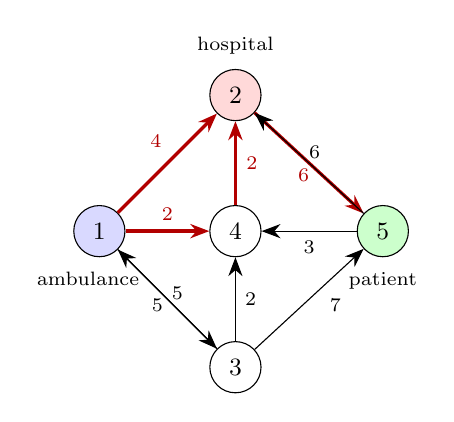
\begin{tikzpicture}[scale=0.72,>={Stealth[length=2.4mm]}]
  \tikzset{vtx/.style={circle,draw,minimum size=6.5mm,inner sep=0.5pt,font=\small}}
  \node[vtx,fill=blue!15] (1) at (0,2.4) {$1$};
  \node[vtx,fill=red!15]  (2) at (2.4,4.8) {$2$};
  \node[vtx]              (3) at (2.4,0)   {$3$};
  \node[vtx]              (4) at (2.4,2.4) {$4$};
  \node[vtx,fill=green!20](5) at (5,2.4)  {$5$};
  \node[font=\scriptsize,anchor=north] at (-0.2,1.85) {ambulance};
  \node[font=\scriptsize,anchor=south] at (2.4,5.35) {hospital};
  \node[font=\scriptsize,anchor=north] at (5,1.85) {patient};
 
  \draw[->,very thick,red!70!black] (1) -- node[font=\scriptsize,above left,pos=0.55] {$4$} (2);
  \draw[->] (1) -- node[font=\scriptsize,below,pos=0.4] {$5$} (3);
  \draw[->,very thick,red!70!black] (1) -- node[font=\scriptsize,above,pos=0.5] {$2$} (4);
  \draw[->,very thick,red!70!black] (2) -- node[font=\scriptsize,below,pos=0.45] {$6$} (5);
  \draw[->] (3) -- node[font=\scriptsize,above,pos=0.4] {$5$} (1);
  \draw[->] (3) -- node[font=\scriptsize,right,pos=0.5] {$2$} (4);
  \draw[->] (3) -- node[font=\scriptsize,below right,pos=0.6] {$7$} (5);
  \draw[->,very thick,red!70!black] (4) -- node[font=\scriptsize,right,pos=0.5] {$2$} (2);
  \draw[->] (5) -- node[font=\scriptsize,above,pos=0.45] {$6$} (2);
  \draw[->] (5) -- node[font=\scriptsize,below,pos=0.5] {$3$} (4);
\end{tikzpicture}
\caption{The $5$-vertex, $10$-arc toy network of the tool (Section~\ref{sec:toy}), with arc
costs. Bold arcs form the two optimal ambulance$\,\to\,$patient paths
$1\to2\to5$ and $1\to4\to2\to5$, both of cost $10$; the optimal patient$\,\to\,$hospital path
$5\to4\to2$ (dashed bold in the tool's rendering) costs $3+2=5$.}
\label{fig:toy}
\end{figure}

Figure~\ref{fig:toy} shows the network used throughout the project as its running example:
$5$ vertices, $8$ roads, and $10$ arcs after splitting the two-way roads. With the time
criterion and unit multipliers $\omega_{\text{traffic}}=\omega_{\text{road works}}=2$,
$\omega_{\text{gravel}}=3$, the cost vector is
$c=(4,5,2,6,5,2,7,2,6,3)^{\!\top}$ for the variables
$(x_{12},x_{13},x_{14},x_{25},x_{31},x_{34},x_{35},x_{42},x_{52},x_{54})$, and the two
right-hand sides are $b_{A\to P}=(1,0,0,0,-1)^{\!\top}$ and
$b_{P\to H}=(0,-1,0,0,1)^{\!\top}$. Solving~\eqref{eq:ip} with GLPK returns
$Z_{A\to P}=10$ (attained \emph{twice}, by $x_{12}=x_{25}=1$ and by
$x_{14}=x_{42}=x_{25}=1$) and $Z_{P\to H}=5$ (attained by $x_{54}=x_{42}=1$). At the
default parameters ($1$\,m cells, $10$\,km/h) these are $3.6$\,s and $1.8$\,s of absolute
travel time.

\section{$A^{\star}$ search with a Manhattan heuristic}
\label{sec:astar}

For interactive single-pair queries the tool also implements $A^{\star}$ search~\cite{hnr68}: nodes
are expanded in increasing order of $f(n)=g(n)+h(n)$, where $g(n)$ is the cost incurred from
the source to $n$ and $h(n)$ estimates the remaining cost to the target. Dijkstra's
algorithm~\cite{dijkstra59} is the special case $h\equiv 0$; $A^{\star}$ is preferable here because
exactly one target matters, whereas Dijkstra necessarily computes distances to all
vertices. Both algorithms are complete on finite graphs with nonnegative costs.

The heuristic is the Manhattan distance to the target, $h(n)=\dman(n,t)$: on a rectangular
street plan, the length of \emph{any} route between two vertices is at least their
$\ell_1$-distance~\cite{krause86}, so the estimate is structurally reliable rather than
merely plausible.

\begin{proposition}[Admissibility and consistency of the Manhattan heuristic]
\label{prop:heuristic}
For both criteria of Section~\ref{sec:model}, $h(n)=\dman(n,t)$ is admissible, i.e.\
$h(n)\le \mathrm{dist}(n,t)$ for all $n$, and consistent, i.e.\ $h(u)\le w(u,v)+h(v)$ for
every arc $(u,v)$.
\end{proposition}
\begin{proof}
Every arc $a=(u,v)$ satisfies $w_a \ge \dman(u,v)$: under the length criterion equality
holds by construction; under the time criterion
$w_a=1+\sum_{\gamma\in a}\omega_\gamma \ge k_a+1 > k_a \ge \dman(u,v)$, where $k_a$ is the
number of cells of $a$'s road, which any connected cell chain between $u$ and $v$ must at
least cover. Summing along any $n\!\to\!t$ path and applying the triangle inequality of the
$\ell_1$ metric gives $\mathrm{dist}(n,t)\ge\dman(n,t)$: admissibility. Consistency follows
from the same triangle inequality,
$\dman(u,t)\le\dman(u,v)+\dman(v,t)\le w(u,v)+h(v)$.
\end{proof}

Consequently, $A^{\star}$ with this heuristic is optimal (it returns minimum-cost paths) on our
networks under both criteria~\cite{hnr68,dechterpearl85}. The implementation maintains open
lists, parent pointers, and $g$-scores in dictionaries over grid coordinates and resolves
each road's cost by a lookup keyed by the vertex pair; on all instances of
Section~\ref{sec:exp} its outputs agreed with the IP optima.

\section{Sensitivity analysis}
\label{sec:sens}

The travel-time weights of a road network are volatile: traffic builds up and dissipates,
road works appear and end. It is therefore natural to ask, for each edge $e$ of the current
solution, \emph{how much its cost may change before the optimal route changes}. The tool
answers this with an integer sensitivity analysis: the perturbations applied are the integer
increments and decrements of an edge's relative cost, matching the granularity at which the
add-on multipliers themselves can be edited. Throughout, let $p_{\text{old}}$ be the current
optimal $s\!\to\!t$ path of value $Z$.

\subsection{Perturbing an edge on the optimal path}

\begin{proposition}[Threshold for cost increases]
\label{prop:inc}
Let $e\in p_{\text{old}}$ and let
$M_e=\min\{C(P) : P \text{ an $s\!\to\!t$ path with } e\notin P\}$ (if no such $P$ exists,
set $M_e=\infty$). For an integer increase $\delta\ge 0$ of $c_e$:
\begin{enumerate}
  \item[(i)] the perturbed optimum is
        $Z(\delta)=\min\{Z+\delta,\;M_e\}$, a concave piecewise-linear function of $\delta$
        with a single breakpoint (Figure~\ref{fig:vf}a);
  \item[(ii)] $p_{\text{old}}$ remains optimal if and only if
        $0\le\delta\le\Delta c^{\max}_e$, where
        \begin{equation}
        \label{eq:threshold}
          \Delta c^{\max}_e \;=\; M_e - Z \;\ge\; 0,
        \end{equation}
        with ties possible at $\delta=\Delta c^{\max}_e$; for
        $\delta=\Delta c^{\max}_e+1$ the strictly better alternative avoiding $e$ takes
        over.
\end{enumerate}
\end{proposition}
\begin{proof}
Paths avoiding $e$ are unaffected by $\delta$, so their best value stays $M_e$; every path
through $e$ shifts up by exactly $\delta$, and the best of them is $p_{\text{old}}$ itself
with $C(p_{\text{old}})+\delta=Z+\delta$. Hence
$Z(\delta)=\min\{Z+\delta,M_e\}$, and $Z+\delta\le M_e$ iff $\delta\le M_e-Z$.
\end{proof}

If $e$ is a bridge (every $s\!\to\!t$ path uses $e$), then $M_e=\infty$ and the tolerance is
unbounded: the network can absorb any increase of $c_e$ without rerouting.

\subsection{Perturbing an edge off the optimal path}

\begin{proposition}[Threshold for cost decreases]
\label{prop:dec}
Let $e\notin p_{\text{old}}$ and let $M'_e=\min\{C(P):P\text{ an $s\!\to\!t$ path with }
e\in P\}$. For an integer decrease of $c_e$ by $\delta\ge 0$ (bounded below by the minimum
achievable cost $\ell_e$ of $e$, i.e.\ $c_e-\delta\ge\ell_e$): the perturbed optimum is
$Z(\delta)=\min\{Z,\;M'_e-\delta\}$, again concave piecewise-linear
(Figure~\ref{fig:vf}b), and $p_{\text{old}}$ remains optimal iff
$0\le\delta\le\Delta c^{\max\!-}_e$ with
$\Delta c^{\max\!-}_e = Z - M'_e \ge 0$.
At $\delta=\Delta c^{\max\!-}_e$ a path through $e$ ties with $p_{\text{old}}$; beyond it,
each further unit of reduction decreases the optimum by exactly one unit along the new path
(which traverses $e$ once). For the time criterion,
$\ell_e=k_e+1$ where $k_e$ is the number of cells of $e$'s road (all multipliers at their
default $\omega=1$); in particular the geometric floor
$\dman(u_e,v_e)\le\ell_e$ from Section~\ref{sec:astar} bounds any reduction.
\end{proposition}
\begin{proof}
Symmetric to Proposition~\ref{prop:inc}: the best path through $e$ now has value
$M'_e-\delta$ while all others, including $p_{\text{old}}$, keep their costs; the minimum
of the two families gives $Z(\delta)$ and the crossing point $Z-M'_e$. Once
$M'_e-\delta<Z$ the optimum uses $e$, and decreasing $\delta$ further lowers the value one
unit per unit since $e$ is traversed once. The floor $\ell_e$ holds because multipliers are
integers $\ge 1$.
\end{proof}

\begin{figure}[t]
\centering
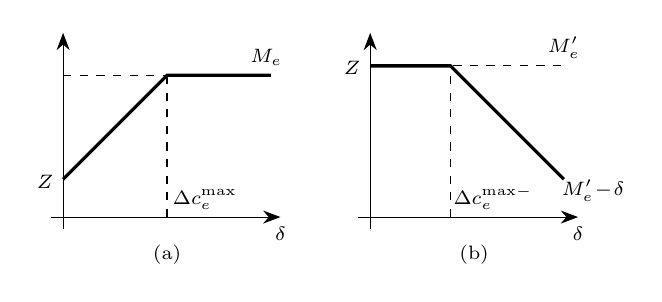
\begin{tikzpicture}[scale=0.6,>={Stealth[length=2.2mm]}]
  \draw[->] (-0.25,0) -- (4.6,0) node[font=\scriptsize,below] {$\delta$};
  \draw[->] (0,-0.25) -- (0,3.9);
  \draw[very thick] (0,0.8) -- (2.2,3.0) -- (4.4,3.0);
  \draw[dashed] (2.2,0) -- (2.2,3.0);
  \node[font=\scriptsize,above] at (3.0,-0.05) {$\Delta c^{\max}_e$};
  \draw[dashed] (0,3.0) -- (4.4,3.0);
  \node[font=\scriptsize,left] at (0,0.75) {$Z$};
  \node[font=\scriptsize,above] at (4.3,3.0) {$M_e$};
  \node[font=\scriptsize] at (2.2,-0.8) {(a)};
  \draw[->] (6.25,0) -- (10.9,0) node[font=\scriptsize,below] {$\delta$};
  \draw[->] (6.5,-0.25) -- (6.5,3.9);
  \draw[very thick] (6.5,3.2) -- (8.2,3.2) -- (10.6,0.8);
  \draw[dashed] (8.2,0) -- (8.2,3.2);
  \node[font=\scriptsize,above] at (9.1,-0.05) {$\Delta c^{\max\!-}_e$};
  \draw[dashed] (6.5,3.2) -- (10.6,3.2);
  \node[font=\scriptsize,left] at (6.5,3.15) {$Z$};
  \node[font=\scriptsize,above] at (10.6,3.15) {$M'_e$};
  \node[font=\scriptsize,below right] at (10.35,1.0) {$M'_e\!-\!\delta$};
  \node[font=\scriptsize] at (8.7,-0.8) {(b)};
\end{tikzpicture}
\caption{The value function of the perturbed problem. (a) Increasing the cost of an edge
$e$ on the optimal path: $Z(\delta)=\min\{Z+\delta,\,M_e\}$ with breakpoint
$\Delta c^{\max}_e=M_e-Z$. (b) Decreasing the cost of an edge off the optimal path:
$Z(\delta)=\min\{Z,\,M'_e-\delta\}$ with breakpoint $\Delta c^{\max\!-}_e=Z-M'_e$, until the
floor $\ell_e$ of $e$ is reached.}
\label{fig:vf}
\end{figure}

\subsection{Locating the integer threshold by binary search}

The thresholds of Propositions~\ref{prop:inc} and~\ref{prop:dec} can be found by increasing
(respectively decreasing) the edge cost in steps of one unit and re-solving
model~\eqref{eq:ip} after each step until the returned optimum signals a reroute. This
linear scan requires up to $N$ IP re-solves, where $N$ is an a priori bound on the relevant
perturbation range (e.g.\ the distance of $c_e$ from its extreme achievable value). Both
value functions of Figure~\ref{fig:vf} are monotone after their single breakpoint, so the
``still optimal'' predicate is \emph{monotone} in $\delta$, and binary search applies.

\begin{algorithm}[t]
\caption{Integer sensitivity threshold via binary search.}
\textbf{Input:} solved instance $(A,b,c)$ with optimal value $Z$; edge $e$; bound $N$;
direction $d\in\{+1,-1\}$.\\
\textbf{Output:} $\Delta c^{\max}_e$ (increase case $d=+1$) or $\Delta c^{\max\!-}_e$
(decrease case $d=-1$).
\begin{enumerate}
  \item $lo\gets 0$; $hi\gets N$.
  \item \textbf{while} $lo<hi$ \textbf{do}
  \item \quad $mid\gets\lceil(lo+hi+1)/2\rceil$.
  \item \quad solve~\eqref{eq:ip} with $c_e$ replaced by $c_e+d\cdot mid$; let $Z(mid)$ be
        its optimal value.
  \item \quad \textbf{if} $Z(mid)=Z+d\cdot mid$ \textbf{then} $lo\gets mid$
        \textbf{else} $hi\gets mid-1$.
  \item \textbf{return} $\Delta\gets lo$.
\end{enumerate}
\end{algorithm}

The predicate in line~5 compares \emph{objective values} only---$Z(\delta)=Z+\delta$ in the
increase case, $Z(\delta)=Z$ in the decrease case---which by
Propositions~\ref{prop:inc} and~\ref{prop:dec} holds exactly up to the threshold and fails
afterwards; this makes the test robust to ties (at $\delta=\Delta c^{\max}_e$ the solver may
return either of the tied paths, but the optimal \emph{value} is unambiguous). The loop
performs at most $\lceil\log_2 N\rceil$ IP re-solves.

\begin{remark}[A certificate of uniqueness]
\label{rem:unique}
If, for \emph{every} edge $e$ of $p_{\text{old}}$, the cost of $e$ can be driven all the way
to its maximum achievable value without the optimal route changing (i.e.\ the tolerance of
$e$ covers its entire admissible range), then $p_{\text{old}}$ is the \emph{unique} optimal
$s\!\to\!t$ path. Indeed, any simple alternative path either strictly contains
$p_{\text{old}}$'s arc set (and is costlier, by positivity of the costs) or omits some edge
$e\in p_{\text{old}}$, in which case its cost is at least $Z+\Delta c^{\max}_e>Z$. Running
the sensitivity analysis over all edges of the incumbent path therefore doubles as a
uniqueness test.
\end{remark}

\section{Experimental evaluation}
\label{sec:exp}

\subsection{Tool and instances}

All experiments were run with the project's tool: a Tkinter-based graphical application in
which the user draws the network, selects the criterion, checks connectivity, solves the
two legs (IP or $A^{\star}$), and applies the sensitivity analysis per edge; instances are stored as
plain-text files listing vertices, edge cells, penalty categories with their multipliers,
and directionalities. Table~\ref{tab:instances} summarizes the five benchmark instances:
grid sizes from $10\times10$ to $100\times100$ cells, $5$ to $28$ vertices, $8$ to $32$
roads (10 to 64 arcs after splitting two-way roads), and both criteria.

\begin{table}[t]
\centering
\caption{The five benchmark instances. $|E|$ counts roads, $|\mathcal{A}|$ the arcs after
splitting two-way roads; $Z$ are the relative optimal costs of the two legs as computed by
the IP (GLPK), cross-validated with Dijkstra's algorithm and with $A^{\star}$ (agreement on all
values and paths). The optima of E3 and E5 were produced with the same model data by an
independent shortest-path implementation, which coincides with the IP optimum by
Proposition~\ref{prop:tu}.}
\label{tab:instances}
\footnotesize
\setlength{\tabcolsep}{4pt}
\begin{tabular}{@{}llrrrrcrr@{}}
\toprule
Inst. & Grid & $|V|$ & $|E|$ & $|\mathcal{A}|$ & Crit. & $Z_{A\to P}$ & $Z_{P\to H}$ \\
\midrule
E1 & $10\times10$  & 5  & 8  & 10 & time   & 10 & 5 \\
E2 & $30\times30$  & 14 & 16 & 26 & length & 24 & 52 \\
E3 & $20\times20$  & 9  & 12 & 24 & time   & 42 & 32 \\
E4 & $50\times50$  & 28 & 32 & 64 & time   & 205 & 258 \\
E5 & $100\times100$& 23 & 27 & 54 & length & 193 & 271 \\
\bottomrule
\end{tabular}
\end{table}

On E1 (Figure~\ref{fig:toy}) the ambulance$\,\to\,$patient leg has the two tied optima of
cost $10$ discussed in Section~\ref{sec:toy}. On E2, the geometrically shorter
patient$\,\to\,$hospital connection of length $30$ is infeasible because one of its roads is
one-way in the opposite direction, and the optimal feasible path costs $52$---an
illustration of why directionality must be modeled explicitly. On E4, the largest
time-criterion instance, GLPK certifies optima $205$ and $258$ for the two legs, matching
the $A^{\star}$ and Dijkstra solutions.

\subsection{The sensitivity experiment}
\label{sec:sensexperiment}

\begin{figure}[t]
\centering
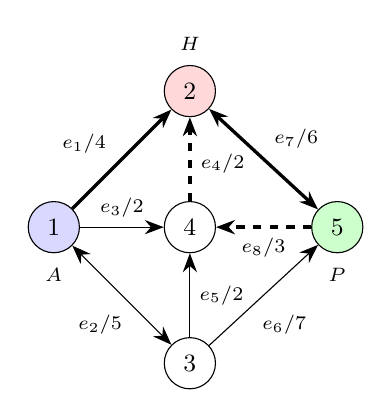
\begin{tikzpicture}[scale=0.72,>={Stealth[length=2.4mm]}]
  \tikzset{vtx/.style={circle,draw,minimum size=6.5mm,inner sep=0.5pt,font=\small}}
  \node[vtx,fill=blue!15] (1) at (0,2.4) {$1$};
  \node[vtx,fill=red!15]  (2) at (2.4,4.8) {$2$};
  \node[vtx]              (3) at (2.4,0)   {$3$};
  \node[vtx]              (4) at (2.4,2.4) {$4$};
  \node[vtx,fill=green!20](5) at (5,2.4)  {$5$};
  \node[font=\scriptsize,anchor=north] at (0,1.85) {$A$};
  \node[font=\scriptsize,anchor=south] at (2.4,5.35) {$H$};
  \node[font=\scriptsize,anchor=north] at (5,1.85) {$P$};
 
  \draw[->,very thick] (1) -- node[font=\scriptsize,above left,pos=0.45] {$e_1/4$} (2);
  \draw[<->] (1) -- node[font=\scriptsize,below left,pos=0.6] {$e_2/5$} (3);
  \draw[->] (1) -- node[font=\scriptsize,above,pos=0.5] {$e_3/2$} (4);
  \draw[->,very thick,dashed] (4) -- node[font=\scriptsize,right,pos=0.45] {$e_4/2$} (2);
  \draw[->] (3) -- node[font=\scriptsize,right,pos=0.5] {$e_5/2$} (4);
  \draw[->] (3) -- node[font=\scriptsize,below right,pos=0.4] {$e_6/7$} (5);
  \draw[<->,very thick] (2) -- node[font=\scriptsize,above right,pos=0.5] {$e_7/6$} (5);
  \draw[->,very thick,dashed] (5) -- node[font=\scriptsize,below,pos=0.5] {$e_8/3$} (4);
\end{tikzpicture}
\caption{The sensitivity experiment network (same vertex layout as
Figure~\ref{fig:toy}); edge labels give the edge id and its time cost. Bold solid arcs form
the optimal ambulance$\,\to\,$patient path $\{e_1,e_7\}$ (cost $10$); bold dashed arcs form
the optimal patient$\,\to\,$hospital path $\{e_8,e_4\}$ (cost $5$).}
\label{fig:sens}
\end{figure}

Figure~\ref{fig:sens} shows the network of the sensitivity study: the same $5$-vertex,
$8$-road network under the time criterion, with two-way roads $e_2$ and $e_7$. There are
four $A\to P$ paths---$\{e_1,e_7\}$ and $\{e_3,e_4,e_7\}$, both of cost $10$, then
$\{e_2,e_6\}$ ($12$) and $\{e_2,e_5,e_4,e_7\}$ ($15$)---and two $P\to H$ paths:
$\{e_7\}$ ($6$) and $\{e_8,e_4\}$ ($5$). The incumbent optima are $\{e_1,e_7\}$ and
$\{e_8,e_4\}$. Table~\ref{tab:sens} reports the thresholds produced by the analysis.

\begin{table}[t]
\centering
\caption{Sensitivity thresholds on the network of Figure~\ref{fig:sens}; ``inc.''/``dec.''
marks an increase/decrease analysis on an edge of the incumbent optimal path (the $A\to P$
incumbent is $\{e_1,e_7\}$, the $P\to H$ incumbent $\{e_8,e_4\}$, and in the decrease
scenario the incumbent is $\{e_7\}$). ``Reroute at $\Delta c^{\max}+1$'' names the
alternative that becomes strictly better one unit past the threshold (its cost under the
unperturbed costs in parentheses). The last row is the decrease case on the modified
instance with a gravel penalty on $e_8$ (making $e_8$ cost $5$ and $\{e_7\}$ optimal at
cost $6$).}
\label{tab:sens}
\footnotesize
\setlength{\tabcolsep}{4pt}
\begin{tabular}{@{}llrrl@{}}
\toprule
Edge & Leg & Type & $\Delta c^{\max}$ & Reroute at $\Delta c^{\max}+1$ \\
\midrule
$e_1$ & $A\to P$ & inc. & $0$ & $\{e_3,e_4,e_7\}$ ($10$) \\
$e_7$ & $A\to P$ & inc. & $2$ & $\{e_2,e_6\}$ ($12$) \\
$e_4$ & $P\to H$ & inc. & $1$ & $\{e_7\}$ ($6$) \\
$e_8$ & $P\to H$ & inc. & $1$ & $\{e_7\}$ ($6$) \\
$e_8$ & $P\to H$ & dec. & $1$ & $\{e_8,e_4\}$ ($7\to5$) \\
\bottomrule
\end{tabular}
\end{table}

All values confirm the closed forms of Propositions~\ref{prop:inc} and~\ref{prop:dec}: for
instance, increasing $c_{e_7}$ leaves both $10$-cost paths through $e_7$ intact while the
best $e_7$-free path costs $12$, hence $\Delta c^{\max}_{e_7}=12-10=2$, and indeed at
$\Delta c_{e_7}=3$ the route flips to $\{e_2,e_6\}$. In the decrease scenario, placing a
gravel penalty on $e_8$ (cost $5$) makes $\{e_7\}$ optimal at cost $6$; one unit of
reduction on $e_8$ produces a tie ($6=6$), two units reroute to $\{e_8,e_4\}$ at cost
$5$---and two units is also the maximum possible reduction, since $e_8$ spans $k=2$ cells
whose multipliers cannot go below the default, i.e.\ its floor is $\ell_{e_8}=k+1=3$.

\begin{table}[t]
\centering
\caption{Linear scan versus binary search for the integer threshold on the edge of
Figure~\ref{fig:sens} analyzed in the project (perturbation bound $N=12$).}
\label{tab:search}
\footnotesize
\setlength{\tabcolsep}{4pt}
\begin{tabular}{@{}lrr@{}}
\toprule
Search strategy & IP re-solves & A priori bound \\
\midrule
Linear scan ($\delta=0,1,2,\dots$) & $9$ & $\le N=12$ \\
Binary search (Algorithm~1)          & $4$ & $\lceil\log_2 12\rceil=4$ \\
\bottomrule
\end{tabular}
\end{table}

Finally, Table~\ref{tab:search} compares the two search modes of Section~\ref{sec:sens} on
the same edge: the linear scan located the threshold at its $8$-th probe and terminated at
the $9$-th ($9$ IP re-solves in total, with bound $N=12$), whereas the binary search located
it in $4$ re-solves---exactly the $\lceil\log_2 12\rceil=4$ guaranteed by the analysis, with
the termination check in its $5$-th iteration. The gap widens with the perturbation bound,
which matters when the analysis is run over all edges of large networks.

\section{Discussion and limitations}
\label{sec:discussion}

\paragraph{What is classical and what is not.}
The ingredients of this project are individually classical: the minimum-cost-flow-type
formulation goes back to Dantzig and Ford--Fulkerson~\cite{dantzig60,fordfulkerson62}, the
total-unimodularity argument is textbook material~\cite{ahuja93,schrijver03}, $A^{\star}$ with a
consistent heuristic is textbook material~\cite{hnr68,dechterpearl85}, and sensitivity
analysis of linear programs is classical~\cite{gass85}. The value of the project lies in
the combination: a single coherent framework in which a drawing becomes a formal IP, both
legs are solved and cross-validated, and a tie-robust, solver-agnostic integer sensitivity
analysis with a binary-search acceleration is layered on top, together with a uniqueness
certificate.

\paragraph{Re-solving versus ranging.}
Because the LP relaxation is exact (Proposition~\ref{prop:tu}), classical LP objective
ranging could in principle read the threshold~\eqref{eq:threshold} directly off the final
simplex basis, without any re-solving; and parametric shortest path algorithms can trace
the full value function for one varying edge in polynomial time~\cite{karporlin81,
youngtarjanorlin91}, with the caveat that the number of breakpoints can be
large~\cite{carstensen83}. The re-solve-based method implemented here trades this
theoretical elegance for two practical advantages: it works with any black-box solver (or
even with the $A^{\star}$ engine) that returns only optimal values, and it extends unchanged to
integer perturbations of the combinatorial add-on structure, where ranging information is
unavailable. A systematic empirical comparison with LP ranging is an obvious next step.

\paragraph{Limitations.}
The experiments are small ($\le 28$ vertices, $\le 64$ arcs) compared with real road
networks, on which specialized techniques dominate~\cite{goldbergharrelson05}; the
travel-time model is static and deterministic, while real travel times are time-dependent
and stochastic~\cite{ordarom90}; and the sensitivity analysis varies one edge at a time,
whereas realistic disruptions (weather, events) move many costs at once. The scenario
itself is the single-vehicle core of a much larger operations problem, in which ambulance
fleet location and dispatch interact~\cite{larson74,brotcorne03,gendreau01}. These are
directions for future work, not obstacles to the present tool's use case: interactive,
educational exploration of the optimization models involved.

\section{Conclusion}
\label{sec:conclusion}

We presented a complete modeling-to-analysis pipeline for a two-leg ambulance routing
scenario on grid-structured city networks: an integer programming formulation with proved
redundancy, integrality, and decomposition properties; an optimally-admissible $A^{\star}$ search
component; and an integer sensitivity analysis whose thresholds are located with
$\lceil\log_2 N\rceil$ re-solves and double as uniqueness certificates. Three independent
solvers agreed on all benchmark instances, and the worked example confirmed every closed
form. The project demonstrates how the classical theory of network flows, polyhedral
integrality, and heuristic search fits together in one small, fully functional application.

\bibliographystyle{unsrt}
\bibliography{bibliography}

\end{document}
